\documentclass[english,12pt,letter]{article}

\usepackage{amsthm}
\usepackage[latin9]{inputenc}
\usepackage{babel}
\usepackage[hmargin=0.9in,vmargin=1.25in]{geometry}
\usepackage{graphicx}
\usepackage{subfigure}
\usepackage[colorlinks=true,citecolor=blue,urlcolor=blue]{hyperref}
\usepackage{amsmath}
\usepackage{amssymb,amsfonts}

\newtheorem{thm}{Theorem}
\newtheorem{lem}{Lemma}
\newtheorem{cor}{Corollary}
\newtheorem{dfn}{Definition}

\newcommand{\Rnot}{\sigma_0}
\newcommand{\Sinf}{x_\infty}
\newcommand{\dom}{{\mathcal D}}
\newcommand{\R}{{\mathbb R}}
\newcommand{\xopt}{x_\text{opt}}
\newcommand{\yopt}{y_\text{opt}}
\newcommand{\ymax}{y_\text{max}}

\DeclareMathOperator\supp{supp}

\begin{document}
\title{Optimal control of an SIR epidemic through finite-time non-pharmaceutical intervention}
\author{
  David I. Ketcheson\thanks{Computer, Electrical, and Mathematical Sciences \& Engineering Division,
King Abdullah University of Science and Technology, 4700 KAUST, Thuwal
23955, Saudi Arabia. (david.ketcheson@kaust.edu.sa)}
}
\maketitle

\abstract{Motivated by the COVID-19 pandemic and responses to it,
we consider the problem of controlling an SIR-model epidemic
by temporarily reducing the rate of contact within a population.
The control takes the form of a multiplicative reduction in the contact rate
of infectious individuals.  The control is allowed to be applied only over
a finite time interval, while the objective is to minimize the total number of
individuals infected in the long-time limit, subject to some cost function for
the control.  We first consider the no-cost scenario and analytically determine
the optimal control and solution.  We then study solutions when a cost of intervention
is included.  Finally, we consider an objective based on flattening the curve
in order to avoid overwhelming the available medical resources.
}

\section{Problem description and assumptions}
The classical SIR model of Kermack \& Mckendrick \cite{kermack1927contribution} is
\begin{subequations} \label{SIR}
\begin{align} 
    x'(t) & = -\beta y(t) x(t) \label{eq:x} \\
    y'(t) & = \beta y(t) x(t) - \gamma y(t) \label{eq:y} \\
    (x(0),y(0)) & \in \dom := \{(x_0,y_0) : x_0 \ge 0, y_0\ge 0, x_0+y_0 \le 1\},
\end{align}
\end{subequations}
where $x(t), y(t)$ represent the susceptible and infected populations
respectively, while the recovered population is $z(t)=1-x(t)-y(t)$.  The region
$\dom$ is forward-invariant and a unique solution exists for all time
\cite{hethcote2000mathematics}.  While
the temporal dynamics of \eqref{SIR} depend on both $\beta$ and $\gamma$, the set
of trajectories depends only on the basic reproduction number 
$\Rnot = \beta/\gamma$.  Dynamics for two values of $\Rnot$ are
shown in Figure \ref{fig:dynamics}.  

The system \eqref{SIR} is at equilibrium if $y(t)=0$.  This equilibrium is stable if and
only if $x(t)\le 1/\Rnot$, a condition referred to as {\em herd immunity}.  If
this condition is not satisfied at
the initial time, then $y(t)$ will first increase until it is, and then decrease,
approaching zero asymptotically.  The SIR model assumes that recovery
confers permanent immunity.

\begin{figure}
    \centering
    \subfigure[$\sigma=3$]{\label{sigma3}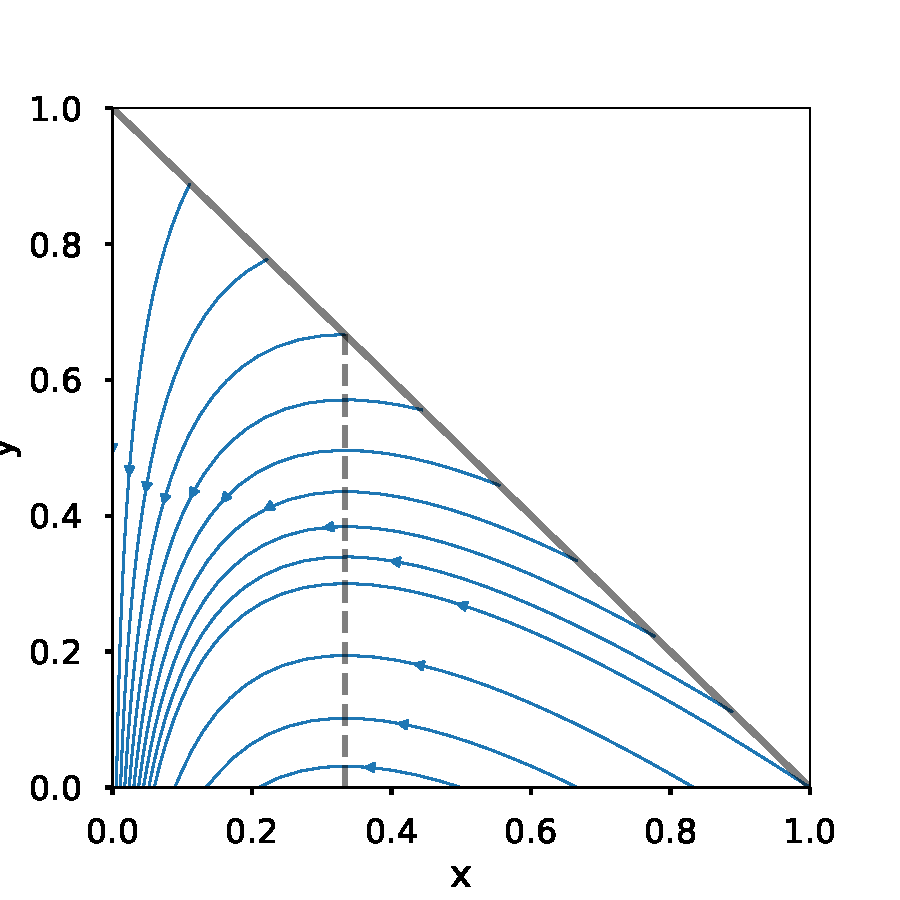
\includegraphics[width=0.49\textwidth]{figures/sigma3.pdf}}
    \subfigure[$\sigma=1.5$]{\label{sigma15}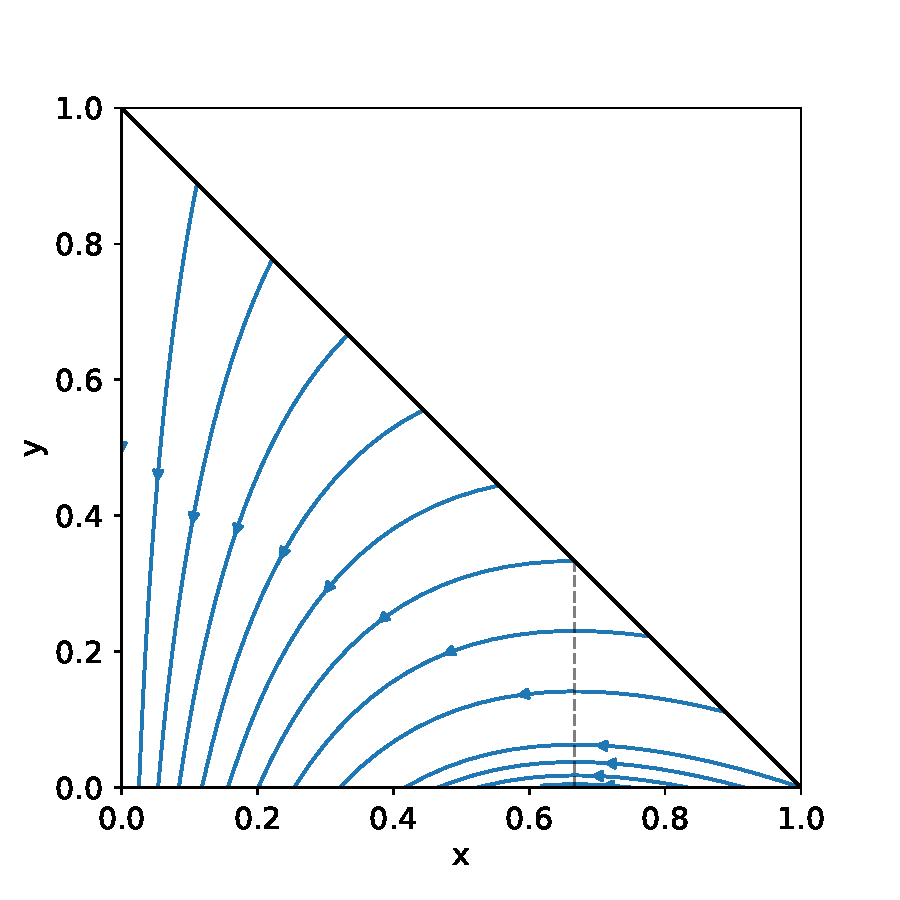
\includegraphics[width=0.49\textwidth]{figures/sigma15.pdf}}
    \caption{Dynamics of SIR model for two values of the basic reproduction number.
            The critical value $x=1/\sigma$ is shown with a dashed line.\label{fig:dynamics}}
\end{figure}

For many diseases affecting humans, herd immunity is achieved
through vaccination of a sufficient portion of the population.  Herein
we assume a vaccine is unavailable, so that herd immunity can only be achieved
through infection and recovery.
Our goal is to minimize $z_\infty := \lim_{t \to \infty} z(t)$, or equivalently
(since $y_\infty=0$)
to maximize the long-time limit of the susceptible fraction:
\begin{align}
    \Sinf = \lim_{t\to\infty} x(t).
\end{align}
This has the effect of minimizing
the number of eventual deaths, which would be proportional to $z_\infty$.

This is equivalent to minimizing the number of deaths, if we assume that
some fixed fraction of the recovered population $z(t)$ dies from the disease.
From the foregoing it is clear that $\Sinf \le 1/\Rnot$.  The difference
$\Rnot-\Sinf$ is referred to as {\em epidemiological overshoot}.

This overshoot can in principle be reduced through
non-pharmaceutical intervention (NPI), which is simply a means to
reduce contact between infected and susceptible individuals.  We model a NPI
control via a time-dependent parameter $q(t)\in[0,1]$ with the SIRq system
\begin{subequations} \label{SIRq}
\begin{align}
    x'(t) & = -(1-q(t))\beta y x \\
    y'(t) & = (1-q(t))\beta y x - \gamma y \\
    (x(0),y(0)) & \in \dom := \{(x_0,y_0) : x_0 \ge 0, y_0\ge 0, x_0+y_0 \le 1\}.
\end{align}
\end{subequations}
An active control $q(t)>0$ reduces the effective reproduction number which is now
given by 
$$\sigma(t) = (1-q(t))\Rnot.$$
This can account for both
population-wide interventions and interventions specific to identified infectious
(or possibly infectious) individuals.  

Typically, an epidemic does not result in substantial {\em permanent} change in the contact rate of
a population.  We therefore assume 
\begin{align} \label{q-shortterm}
    q(t)=0 \text{ for } t>T,
\end{align}
i.e., that intervention can only be applied over a limited time, up to $T$.
Since $x_\infty=1/\sigma_0$ only at the single point $(x=1/\sigma_0,y=0)$, and since 
the $y=0$ axis cannot be reached in a finite time, \eqref{q-shortterm} implies
that any solution must have $x_\infty<1/\sigma_0$.
%In either model \eqref{SIR} or \eqref{SIRq}, the zero-infection axis
%$y=0$ can only be reached after an infinite amount of time. Therefore our
%objective will be to achieve $x_\infty=1/\sigma_0 - \epsilon$ for a prescribed
%value $\epsilon$.

We state the control problem as follows:
\begin{align} \label{eq:basic-problem}
\begin{aligned}
& \text{Given } x_0, y_0, \sigma_0, T, \text{ choose } q(t) \in [0,1] \text{ to minimize }  \\
&     J = -x_\infty(x(T),y(T),\sigma_0) + c_2 \int_0^T L(q(t) dt \\
& \text{ subject to } \eqref{SIRq}.
\end{aligned}
\end{align}
Here $J(x_\infty,q)$ is the objective function that accounts for the desire to
minimize infections as well as a cost of imposing control.


There is a large body of work on compartmental epidemiological models
and control for such models; here we will mention just a few of the most
relevant works.
Optimal control in the SIR model with vaccination has been studied in \cite{kar2011stability}.
Optimal control for an extended SIR model, based on quarantining and isolation
of confirmed or suspected cases was studied in \cite{yan2008optimal}.  
A review of work on optimal control in epidemiology is presented in \cite{sharomi2017optimal},
along with the formulation of the optimal control solution (based on
Pontryagin's maximum principle) for several extensions of the SIR model.
The effect of quarantine or NPI can also be studied through more
detailed compartmental models that include compartments for quarantined individuals,
as has been done for instance in \cite{safi2013dynamics,agusto2013optimal}, or with
sophisticated models incorporating spatial spread and human networks;
see e.g. \cite{ferguson2005strategies}.

The modeling and assumptions in the present work are motivated by the
current COVID-19 epidemic, which so far is being managed through broad
NPIs and without a vaccine.  In order to understand the effects of NPIs
imposed on an entire population, we stick to the simple model \eqref{SIRq}
rather than explicitly modeling quarantined individuals.
Since such population-wide measures cannot be maintained indefinitely, we
invoke the finite-time control assumption \eqref{q-shortterm}.
This assumption is not new (see e.g. \cite{greenhalgh1988some}),
but unlike previous works our objective function is still based on the
long-term outcome (rather than the outcome at time $T$).
This drastically changes the nature of optimal solutions.
In the last section of this work we also consider the goal of avoiding
hospital overflow (through {\em flattening the curve}).

The rest of the paper is organized as follows.  In Section \ref{sec:prelims} we
review results on the exact solution of the SIR model and compute some quantities
that will be central to our results.  In Section \ref{sec:analytic} we state
and prove solutions of \eqref{eq:basic-problem} under certain choices of $J$.
In Section X we illustrate results for other choices of $J$ with computational
examples.

\section{Preliminaries\label{sec:prelims}}

\subsection{Notation}
The control above is given as $q(t)$, but for most purposes it is more
convenient to work with the effective reproduction number, defined as
$$
    \sigma(t) := (1-q(t))\Rnot = (1-q(t))\beta/\gamma.
$$
We will often simply refer to $\sigma(t)$ as the control.

In general, the solution of \eqref{SIRq} depends on the initial data
$(x_0,y_0)$, the control $\sigma(t)$, and time $t$, so it is natural to write
$x(t;\sigma(t),x_0,y_0)$.
In what follows it will be convenient to make a slight abuse of notation and
write $x(t;\sigma(t))$ or $x(t)$ when there is no chance of confusion.

For a fixed reproduction number, the asymptotic susceptible fraction $\Sinf$
can be obtained from the solution $x(t), y(t)$ at any time $t$, since solutions
of \eqref{SIR} move along contours of $\Sinf$.  Thus we will write $\Sinf(x,y)$
or $\Sinf(x,y,\Rnot)$.

\subsection{A formula for $\Sinf$}
In this subsection we consider the solution of the SIR model without
control \eqref{SIR}.
It can be shown that $x(t)$ satisfies (see e.g. \cite{harko2014exact,pakes2015lambert})
$$
    x(t)e^{\Rnot z(t)} = x_0 e^{\Rnot z_0}.
$$
Since $z=1-x-y$ we define
$$
   \mu(x,y,\Rnot) := x(t) e^{-\Rnot(x(t)+y(t))},
$$
which is constant in time for any solution of \eqref{SIR}.
The trajectories in Figure \ref{fig:dynamics} are thus also contours of $\mu$.
Since $y_\infty=0$, we have
$$
    x_\infty = x_0 e^{\Rnot(x_\infty-x_0-y_0)} = \mu(x_0,y_0,\Rnot) e^{\Rnot x_\infty}.
$$
Setting $w=-x_\infty \Rnot$ we have
$$
    we^w = -x_0 \Rnot e^{-\Rnot(x_0+y_0)} = -\mu \Rnot.
$$
Thus $w = W_0(-\mu\Rnot)$ where $W_0$ is the principal branch of Lambert's $W$-function \cite{pakes2015lambert},
and
\begin{align} \label{eq:xinf}
    x_\infty = -\frac{1}{\Rnot}W_0(-\mu \Rnot).
\end{align}
In what follows we will also require the derivatives of $\Sinf$ with respect to $x$ and $y$.
Direct computation gives
\begin{subequations} \label{xinf-grad}
\begin{align}
    \frac{\partial \Sinf}{\partial y(t)} & = -\frac{\Rnot \Sinf}{1-\Rnot \Sinf} \\
    \frac{\partial \Sinf}{\partial x(t)} & = \left(1-\frac{1}{x(t)\Rnot}\right) \frac{\partial \Sinf}{\partial y(t)}
      = \frac{1-\Rnot x(t)}{1-\Rnot \Sinf} \cdot \frac{\Sinf}{x(t)}.
\end{align}
\end{subequations}
Using these expressions we can also compute the rate of change of $\Sinf$ when some
control $\sigma(t)$ is applied:
\begin{align} \label{dxinf-dt}
    \frac{\partial \Sinf}{\partial t} = \frac{\gamma y \Sinf}{1-\Rnot\Sinf}(\Rnot - \sigma(t)).
\end{align}
From this we see that the impact of an intervention on $\Sinf$ is independent of $x(t)$ and
directly proportional to $y(t)$.  This indicates that intervention is more impactful
when there is a larger infected population.
%\begin{align*}
%\frac{d \Sinf}{d\mu} = W'(-\mu \Rnot) = \frac{1}{e^{-\Rnot\Sinf}-\mu \Rnot} > 0,
%\end{align*}
%so $\Sinf$ is a monotone function of $\mu$ and maximizing the former is equivalent to
%maximizing the latter.
%Now
%\begin{align*}
%    \frac{d}{dt} \mu(x(t;\sigma(t)),y(t;\sigma(t)),\Rnot) = (\Rnot-\sigma(t))\gamma y(t;\sigma(t)) \mu(t).
%\end{align*}
%\begin{align*}
%    \frac{\partial \Sinf}{\partial y} & = W'(-\mu\Rnot) \frac{\partial \mu}{\partial y}
%\end{align*}
%
%
%The formulas in this section also hold for the solution of \eqref{SIRq} if
%$q(t)$ is a constant function and $\Rnot$ is replaced in these formulas by
%$\sigma=(1-q)\Rnot$.


%We define the solution operator $\phi_t(\beta,\gamma): \dom \to \dom$ as the map
%that takes an initial condition $(x_0,y_0)$ to the solution $(x(t),y(t))$
%via the solution of \eqref{SIR}.  We further define for $u\in\dom$
%$$
%    x_\infty(u,\sigma) = \lim_{t\to\infty} \phi_t(\sigma,1)u.
%$$
%Observe that each trajectory in Figure \ref{fig:dynamics} is a contour of $x_\infty$.
%Our objective then is to minimize $x_\infty((x(T),y(T)),\Rnot)$.

\subsection{Bounds on $\Sinf$}
Now we turn our attention to the SIR system with control \eqref{SIRq}.

\begin{dfn} ({\bf Admissible control})
We say the control $q(t)$ is admissible if it is piecewise continuous and $0\le q(t) \le 1$.

Equivalently, given a basic reproduction number $\Rnot$, we say a control fuction $\sigma(t)$ is
admissible if it is piecewise continuous and $0\le \sigma(t) \le \sigma_0$ for all $t$.
\end{dfn}

It is straightforward to show that \eqref{SIRq} has a unique solution for all time
for any initial data in $\dom$ and any admissible control, by the same
arguments used for \eqref{SIR}.


By applying the control we can move the solution to a different contour of
$x_\infty(\cdot,\sigma)$.  The next lemma states that applying any control $q>0$ over
any length of time leads to an increase in $x_\infty$.
\begin{lem}
Let $\Rnot>0$ and $u\in\dom$ be given and define $X_\infty = x_\infty(x_0,y_0,\Rnot)$.
Let $\sigma(t)$ be an admissible control such that $\sigma(t)\le \sigma_0$.
Then for $t\ge0$ we have
$$
    x_\infty(x(t;\sigma(t)),y(t;\sigma(t)),\Rnot) \ge X_\infty.
$$
\end{lem}
\begin{proof}
    Dividing \eqref{eq:y} by \eqref{eq:x} gives
    \begin{align} \label{eq:dydx}
        \frac{dy}{dx} = -1 + \frac{1}{\sigma x}.
    \end{align}
    Thus reducing $\sigma$ has the effect of increasing $dy/dx$.
    Since all trajectories flow to the left ($x$ is a decreasing function of $t$),
    this means that the solution trajectory obtained with $\sigma(t)$ lies
    below that obtained with $\sigma_0$, for all $t>0$.  Since
    $\Sinf$ is a decreasing function of $y$, this completes the proof.
\end{proof}

Thus for any admissible control and any initial data we have
$$
\Sinf(x_0,y_0,\Rnot) \le \Sinf(x(T),y(T),\Rnot) \le 1/\Rnot.
$$
%\begin{cor} \label{cor:diff-control}
%Let two control functions $q(t), \hat{q}(t)$ be given with $\hat{q}(t)<q(t)$.
%Then $x_\infty(q)>x_\infty(\hat{q})$.
%\end{cor}

%In the classic SIR model, the asymptotic susceptible fraction $\Sinf$ is
%given as a function of the initial state and of $\Rnot$ by the unique solution 
%in the interval $(0,1/\Rnot)$ of the
%following equation \cite[Eqn. (5.4)]{hethcote1989three}:
%\begin{align} \label{s-infty}
%    1 - z_0 - \Sinf + \frac{1}{\Rnot} \log\left(\frac{\Sinf}{x_0}\right) = 0.
%\end{align}
%
%\begin{thm}
%Let $y_0>0$ and
%let $\Sinf(q) = \lim_{t\to\infty} x(t;q)$ where $x(t;q)$ denotes the solution of
%\eqref{SIRq} subject to \eqref{q-shortterm}.  Then $\Sinf\le 1/\sigma$.
%\end{thm}
%\begin{proof}
%Due to condition \eqref{q-shortterm}, as $t \to \infty$ the solution of \eqref{SIRq}
%must tend to a stable equilibrium point of \eqref{SIR}.  But the stable equilibrium
%points of \eqref{SIR} satisfy $x \le 1/\sigma$.
%\end{proof}

\subsection{Infinite-time control}
In this section only, we consider controls that reach the optimal value $\Sinf = 1/\Rnot$.
This is achieved only at $(x,y)=(1/\Rnot,0)$, a state that cannot be reached
from any other state without imposing some control, and which in any case can
only be reached after an infinite time.  Thus we momentarily set aside the restriction
\eqref{q-shortterm} and consider controls over the semi-infinite interval $t\in[0,\infty)$.
We assume that $x_0\ge1/\Rnot$, since otherwise the maximum achievable value of $\Sinf$
is $x_0$, which is achieved by taking $q(t)=1$ for all $t$.
We also take $L=0$ so that an optimal control is any control satisfying
$$
    \lim_{t \to \infty} x(t,\sigma(t)) = 1/\Rnot.
$$
There are infinitely many such controls.  Two are particularly simple and
are of interest.

The first is a constant control $q(t) = q^*(x_0, y_0, \Rnot)$, with
corresponding constant reproduction number $\sigma^*=(1-q^*)\Rnot$.
By \eqref{eq:xinf} we must have $\Sinf(x_0,y_0,\sigma^*)=1/\Rnot$, so $\sigma^*$ is the solution of
$$
    W_0(-\mu(x_0,y_0,\sigma_*)\sigma_*) = -\frac{\sigma^*}{\sigma_0}.
$$

The second is a bang-bang control in which
$$
    \sigma(t) = \begin{cases} \Rnot & x>1/\Rnot \\ 0 & x=\Rnot. \end{cases}
$$
The response for each of these controls is shown for a specific example in
Figure \ref{fig:two-controls}.
\begin{figure}
    \centering
    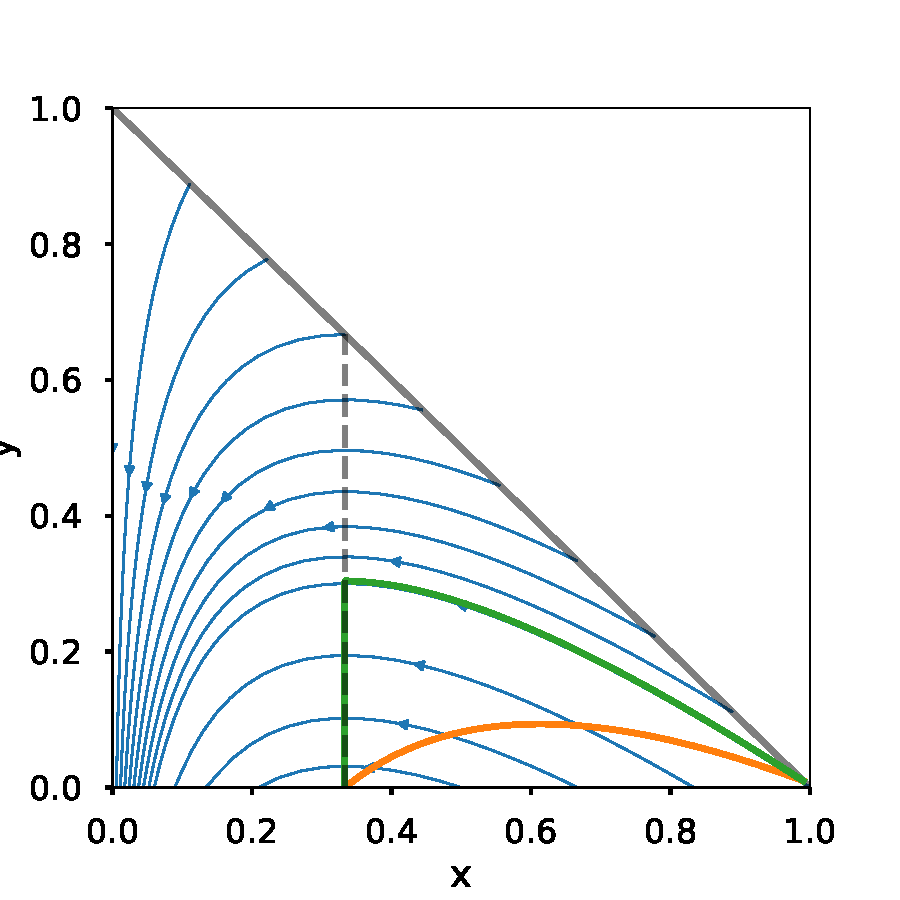
\includegraphics[width=0.5\textwidth]{figures/twocontrols.pdf}
    \caption{Two infinite-time controls that give $\Sinf=1/\Rnot$.  Here $\Rnot=3$ and
        $(x_0,y_0)=(0.99,0.01)$.  For the constant control, $q(t)=q^*\approx0.4557$.\label{fig:two-controls}}
\end{figure}



\subsection{Formulation as a boundary value problem}
Standard application of Pontryagin's maximum principle gives necessary conditions
for a solution of \eqref{eq:basic-problem}.  The Hamiltonian for this problem is
$$
    H(t) = -\lambda_1(t) \gamma \sigma(t) y(t) x(t) + \lambda_2(t)\gamma y(t)(\sigma(t) x(t) - 1) + c_2 L(q).
$$
The necessary conditions for an optimal control consist of $\eqref{SIRq}$ together with
\begin{subequations}\label{lambda-odes}
\begin{align} 
    \lambda_1'(t) & = -\frac{\partial H}{\partial x} = (\lambda_1-\lambda_2)\gamma\sigma(t) y \\
    \lambda_2'(t) & = -\frac{\partial H}{\partial y} = (\lambda_1-\lambda_2)\gamma\sigma(t) x + \lambda_2 \gamma \\
    \lambda_2(T) & = -\frac{\partial \Sinf(T)}{\partial x} = \frac{\partial }{\partial y(T)} (-x_\infty(x(T),y(T),\sigma_0) \\
    \lambda_1(T) & = -\frac{\partial \Sinf(T)}{\partial y} =\frac{\partial }{\partial x(T)} (-x_\infty(x(T),y(T),\sigma_0) = \left(1-\frac{1}{x(T)\sigma_0}\right)\lambda_2(T),
\end{align}
\end{subequations}
as well as the condition $\partial H/\partial \sigma = 0$, which reads:
\begin{align*}
    \sigma(t) = \sigma_0 - \frac{(\lambda_2(t)-\lambda_1(t))\gamma y x}{2c_2}.
\end{align*}
We additionally impose the constraint $0\le \sigma(t) \le \sigma_0$, yielding
\begin{align} \label{eq:sigma-c2}
    \sigma(t) = \max\left(0,\min\left(\sigma_0,\sigma_0 - \frac{(\lambda_2(t)-\lambda_1(t))\gamma y x}{2c_2}\right)\right).
\end{align}
The final conditions for $\lambda_{1,2}$ can be computed from \eqref{xinf-grad}.

In fact, these conditions are also sufficient for optimality.
\begin{thm}
    Let $x_0, y_0, \beta, \gamma, T$ be given.  Then if $\sigma(t)$ is an admissible control and
    $\sigma(t), x(t), y(t), \lambda_1(t), \lambda_2(t)$ satisfy \eqref{SIRq}, \eqref{lambda-odes},
    and \eqref{eq:sigma-c2}, then $\sigma(t)$ is an optimal control for \eqref{SIRq}.
\end{thm}
\begin{proof}
    Since $\Sinf$ is a continuously differentiable function of $x, y$, $\sigma(t)$ is piecewise
    continuous, and \eqref{SIRq} has a unique solution for every admissible control,
    this follows from standard results in control theory; see e.g. \cite[Thm. 3.4.1]{speyer2010primer}.
\end{proof}

\section{Optimal finite-time control\label{sec:analytic}}
In this section we use analysis and computation to investigate solutions of the
optimal control problem through the boundary value problem just derived.

\subsection{Zero-cost control}
We start by investigating the control problem \eqref{eq:basic-problem} when $c_2=0$
(i.e., when the goal of increasing $x_\infty$ completely
trumps any associated costs or other concerns).  Then \eqref{eq:basic-problem} becomes
\begin{align} \label{eq:no-cost-problem}
\begin{aligned}
& \text{Given } x_0, y_0, \sigma_0, T, \text{ choose an admissible control} q(t) \\
& \text{ to minimize }  J = -x_\infty(x(T),y(T),\sigma_0) \\
& \text{ subject to } \eqref{SIRq}.
\end{aligned}
\end{align}
This problem can be reformulated as a minimum-time control problem.  Suppose
that the optimal control for \eqref{eq:no-cost-problem} leads to the terminal
state $(x(T),y(T)) = (\xopt,\yopt)$.  There cannot be a
control that gives $(x(t^*),y(t^*)) = (\xopt,\yopt)$ for some $t^*<T$, since then
we could obtain a better solution by using that control combined with the choice
$q(t)=1$ for $t>t^*$.  In other words,
the optimal control is the one that arrives at $(\xopt,\yopt)$ in the shortest time,
starting from $(x_0,y_0)$.

Since the problem can be formulated as a minimum-time problem, we know that
there must exist an optimal control of bang-bang type.  This motivates the
following lemma.

\begin{lem} \label{lem:shortest-path}
Let $(x_0,y_0)$ and $(x_1,y_1)$ be given such that $x_0, x_1 \ge 1/\Rnot$ and
$\Sinf(x_0,y_0,\Rnot)\ge\Sinf(x_1,y_1,\Rnot)$.
Let $\sigma(t)$ be a bang-bang control such that $(x(t_1;x_0,y_0,\sigma(t)),y(t_1;x_0,y_0,\sigma(t)))=(x_1,y_1)$
for some $t_1\ge0$.  Then the minimum value of $t_1$ is achieved by taking
\begin{align}
    q(t) & = \begin{cases}  
        0 & t<t^* \\
        1 & t^* \le  t \le T,
    \end{cases}
\end{align}
where $t^*$ satisfies $x(t^*;x_0,y_0,\Rnot)=x_1$.
\end{lem}
\begin{proof}
Since $q(t)$ is a bang-bang control, the trajectory $(x(t;q(t)),y(t;q(t)))$ 
consists of a sequence of segments each of which is a solution of
\eqref{SIRq} with $\sigma=0$ (traveling directly downward) or with $\sigma=\sigma_0$
(traveling along a contour of $x_\infty$).  Some trajectories of this type are
illustrated in Figure \ref{fig:bangbangtraj}.  Notice that each trajectory must
traverse the same distance in the x-direction; since $x'(t)=-\beta xy$ this
travel is faster at larger $y$ values.  Meanwhile, the total length of all the
downward ($\sigma=0$) segments is the same for any trajectory, and since for
these segments $y'(t) = -\gamma y$, travel is again faster at larger $y$ values.
The control given in the lemma makes all these traversals at the largest
possible values of $y$, so it arrives in the shortest time.
\end{proof}

\begin{figure}
    \centering
    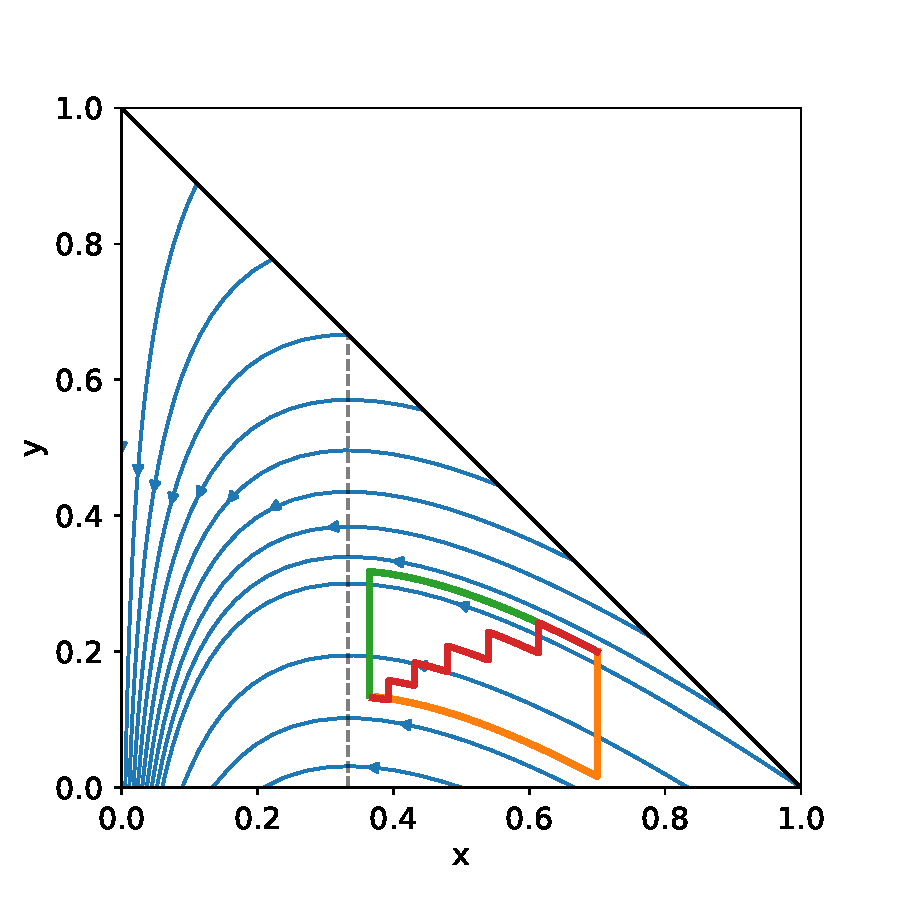
\includegraphics[width=0.5\textwidth]{figures/threepaths.pdf}
    \caption{Three different paths between two states, each obtained
    with a bang-bang control.  The top (green) path arrives in the shortest time.\label{fig:bangbangtraj}}
\end{figure}
%The lemma above holds for the set of all admissible controls, but here we
%only need the result for bang-bang controls.
We can now give the solution of \eqref{eq:no-cost-problem}.
\begin{thm}
An optimal control for \eqref{eq:no-cost-problem} is given by
\begin{align}
    q(t) & = \begin{cases}  
        0 & t<t^* \\
        1 & t^* \le  t \le T,
    \end{cases}
\end{align}
where $t^*=0$ if $x(0)\le1/\sigma_0$ and otherwise $t^*$ is the unique solution of
\begin{align} \label{xtstar}
    x(t^*;\Rnot,x_0,y_0) = \frac{1}{\sigma_0(1-e^{-\gamma(T-t^*)})}.
\end{align}
\end{thm}
\begin{proof}
First, suppose $x(0)\le1/\sigma_0$.  The claimed optimal control gives $x(T)=x_0$, whereas
any other control will give $x(T)<x_0$.  Similarly, we see from \eqref{SIRq} that
the optimal control gives $y(T)=e^{-\gamma T}y_0$ and any other control will
lead to a larger value of $y(T)$.  Since $\Sinf$ is a decreasing function of $y$ and
(for $x<1/\Rnot$) an increasing function of $x$, the proposed control is optimal in this case.

Now suppose $x(0)>1/\sigma_0$.  Taking the limit $c_2\to 0$ in \eqref{eq:sigma-c2} gives
\begin{align}
    \sigma(t) & = \begin{cases} 0 & \lambda_1(t)<\lambda_2(t) \\ \sigma_0 & \lambda_1(t) > \lambda_2(t). \end{cases}
\end{align}
In other words, the solution is a bang-bang control that switches when $\lambda_2-\lambda_1$ changes sign.
Since $\lambda_2(T)>\lambda_1(T)>0$, we have $\sigma(T)=0$.  We can integrate \eqref{lambda-odes} backward from the final
time with $\sigma=0$ to find when $\lambda_1=\lambda_2$.  This yields \eqref{xtstar}.

It remains to show that the optimal control for $t<t^*$ is given by $q=0$.  
Let $(\xopt,\yopt)$ denote the optimal solution at time $T$.  There cannot be a
control that gives $(x(t^*),y(t^*)) = (\xopt,\yopt)$ for some $t^*<T$, since then
we could obtain a better solution by using that control combined with the choice
$q(t)=1$ for $t>t^*$.  In other words,
the optimal control is the one that arrives at $(\xopt,\yopt)$ in the shortest time,
starting from $(x_0,y_0)$.  The result then follows from Lemma \ref{lem:shortest-path}.
\end{proof}

Some optimal solutions for particular instances of \eqref{eq:no-cost-problem}
are shown in Figures \ref{fig:example1} and \ref{fig:diff-time-opt},
all with the same initial data and parameters $\beta, \gamma$ but with different final
times $T$.  Allowing for a longer intervention (larger $T$) makes it possible to reach
a more optimal value of $\Sinf$.

\begin{figure}
    \centering
    \subfigure[Solution and control vs. time]{\label{fig:ex1-time}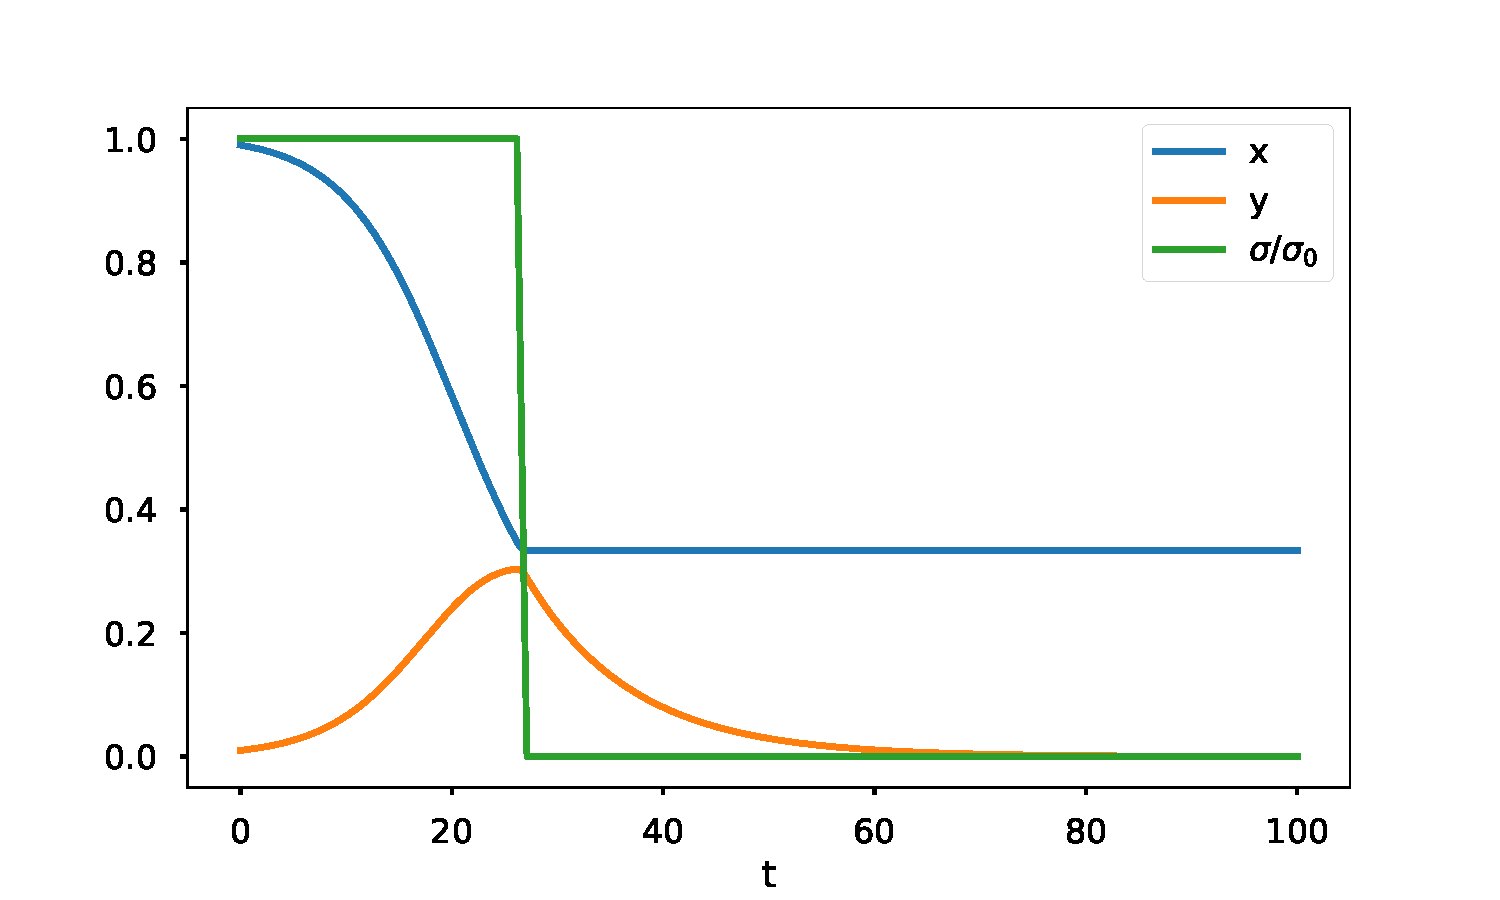
\includegraphics[width=0.65\textwidth]{figures/example1_time.pdf}}
    \subfigure[Trajectory in phase space]{\label{fig:ex1-xy}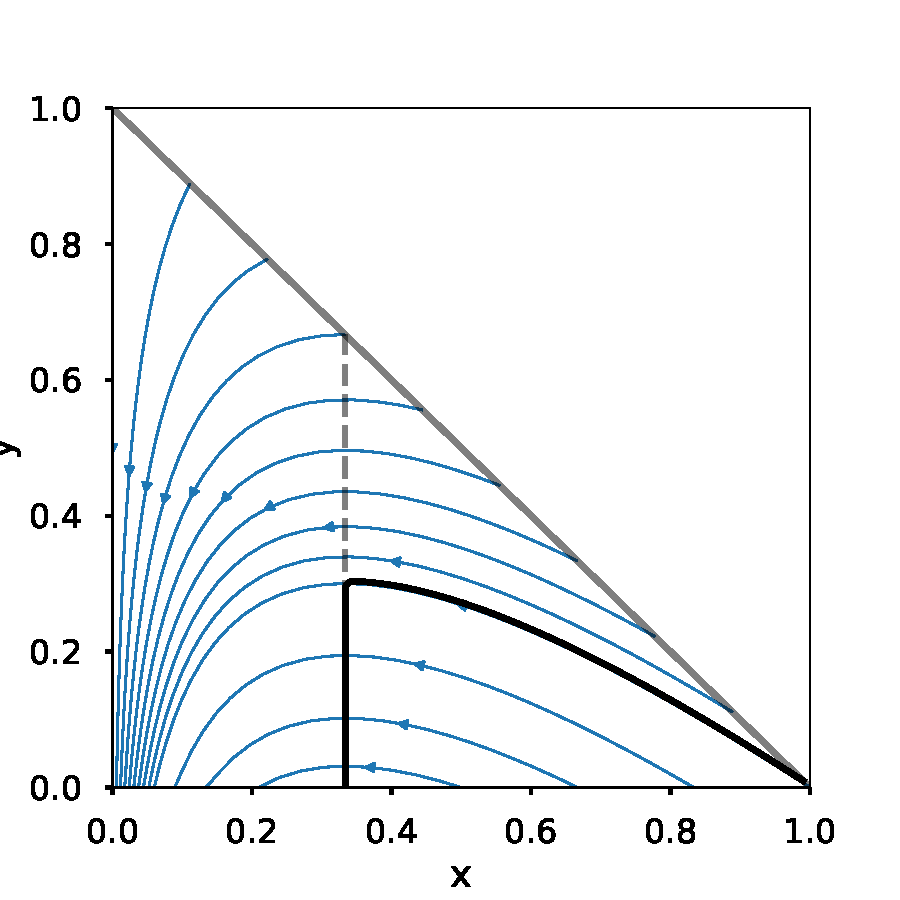
\includegraphics[width=0.34\textwidth]{figures/example1_xy.pdf}}
    \caption{Typical optimal solution.  Here $(x(0),y(0)) = (0.99,0.01)$, $\beta=0.3$, and $\gamma=0.1$.\label{fig:example1}}
\end{figure}

\begin{figure}
    \centering
    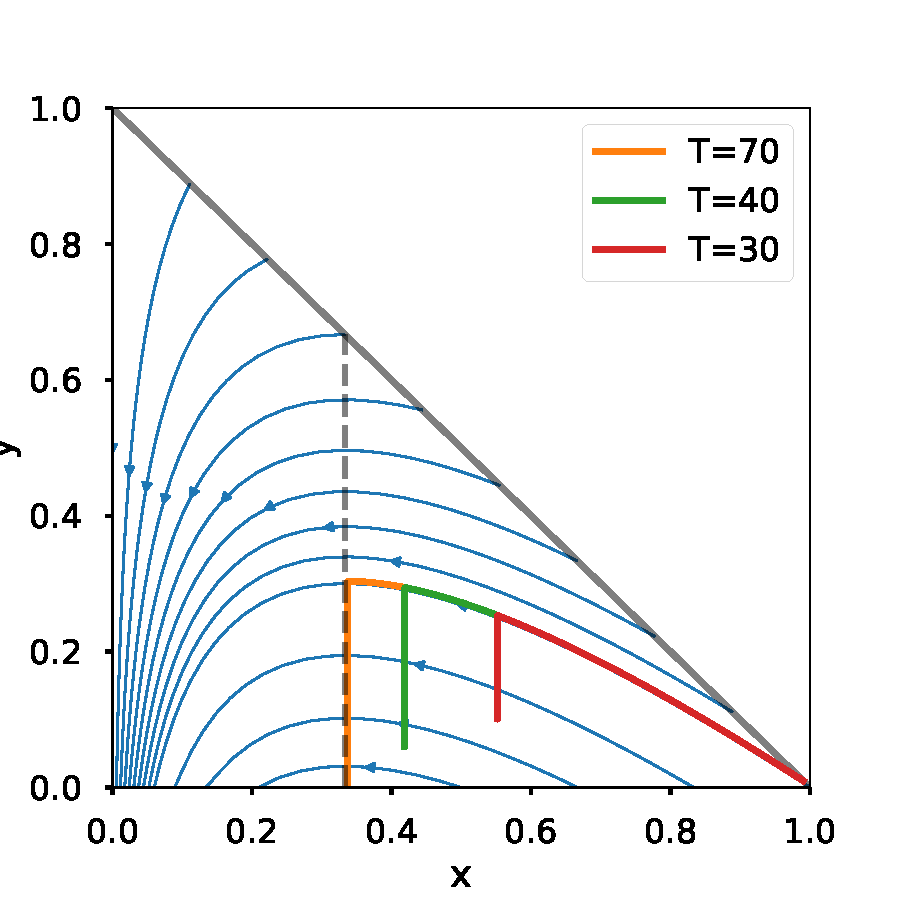
\includegraphics[width=0.5\textwidth]{figures/diff-time-opt.pdf}
    \caption{Optimal solutions starting from the same point $(0.99,0.01)$ but with different
        final times.  A larger value of $T$ allows the system to reach a more optimal state.
        For all solutions, $\beta=0.3$ and $\gamma=0.1$.\label{fig:diff-time-opt}}
\end{figure}


%\subsection{Max-norm cost, infinite-time control}
%If the control can be applied over a semi-infinite time interval, there are many ways
%to achieve the optimal value $\Sinf = 1/\Rnot$.  A natural question is, what is the
%minimum of the maximum control that can be employed to reach this optimum?  We formulate
%the problem as follows:
%\begin{align} \label{eq:max-inf-problem}
%\begin{aligned}
%& \text{Given } x_0, y_0, \sigma_0, \text{ choose } q(t) \in [0,1] \text{ to minimize }  \\
%&     J = -\lim_{t\to\infty} x(t) + c_2 \max_t q(t) \\
%& \text{ subject to } \eqref{SIRq}.
%\end{aligned}
%\end{align}
%For any finite $c_2$, the problem has a unique solution, even though in the limit
%it does not.
%
%\begin{thm}
%In the limit $c_2 \to 0$, the unique optimal control for \eqref{eq:max-inf-problem} tends to
%$$
%    q(t) = 1-\frac{\sigma_*}{\sigma}
%$$
%where
%$$
%    -\frac{1}{\sigma_*} W_0(-\mu(x_0,y_0,\sigma_*)\sigma_*) = \frac{1}{\sigma_0}.
%$$
%\end{thm}
%\begin{proof}
%    The optimality of the given control follows from the fact that $\Sinf \le 1/\Rnot$ and
%    that with this control we attain this bound.  To see the uniqueness, observe that
%    \eqref{eq:dydx} implies that imposing a larger value of $\sigma$ at any time will lead
%    to a solution that lies above the optimal trajectory, and therefore must terminate at
%    a smaller $\Sinf$.
%\end{proof}

Figure \ref{fig:varying_c2} illustrates the optimal no-cost control and also how this control
is modified when a cost for control is included.  We take
$$
    L(q) = q^2
$$
and solve the two-point boundary value problem for a range of values of $c_2$.
Notice that the strength of the optimal control $q(t)$ at early times varies non-monotonically
with $c_2$, first increasing and then decreasing as $c_2$ is reduced.  Indeed, the optimal
control $q(t)$ over the initial time interval is zero in both limits $c_2 \to \infty$ and $c_2 \to 0$.

\begin{figure}
    \centering
    \subfigure[Solution and control vs. time]{\label{fig:varying-c2}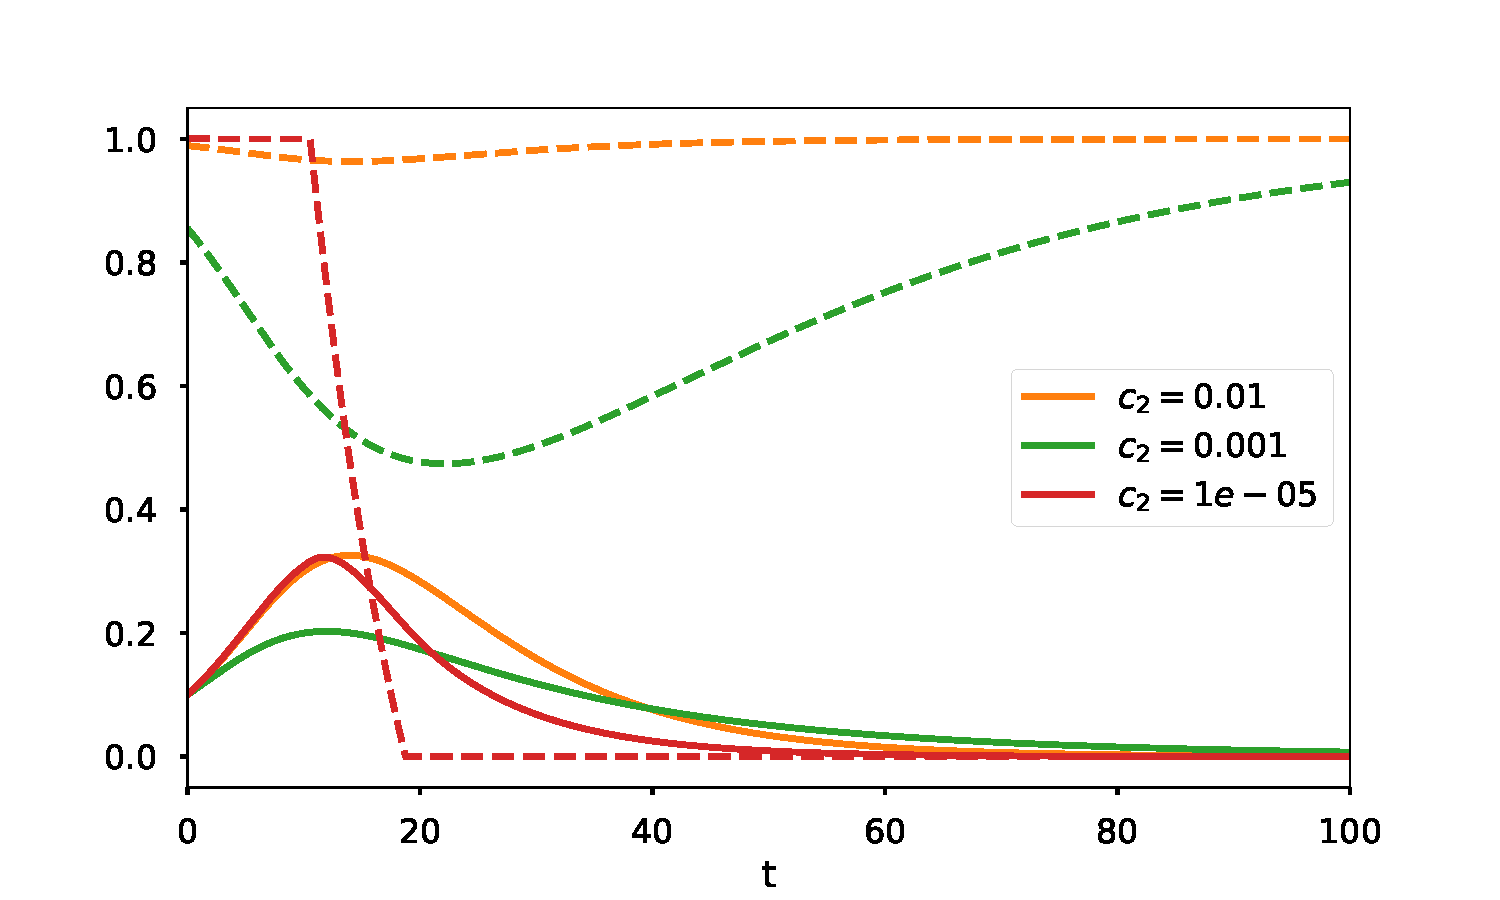
\includegraphics[width=0.65\textwidth]{figures/varying_c2.pdf}}
    \subfigure[Trajectory in phase space]{\label{fig:varying-cs-xy}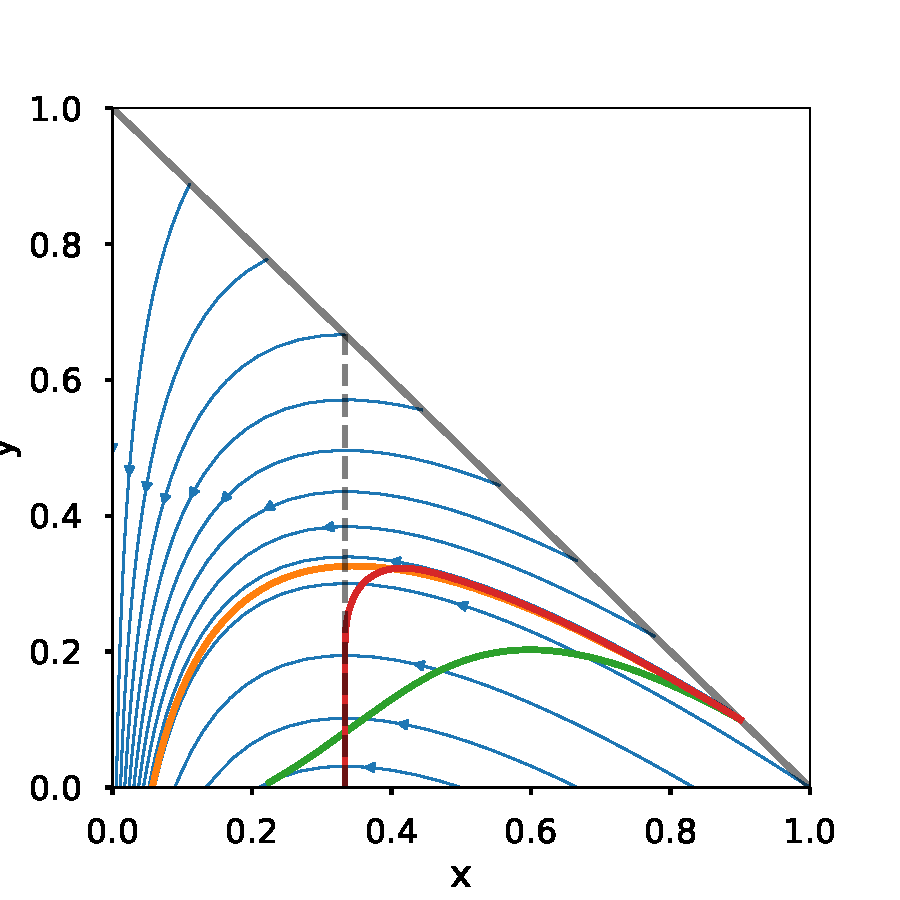
\includegraphics[width=0.34\textwidth]{figures/varying_c2_xy.pdf}}
    \caption{Optimal solutions with different running cost.  Here $(x(0),y(0)) = (0.99,0.01)$, $\beta=0.3$, $\gamma=0.1$, and $T=100$.\label{fig:varying_c2}}
\end{figure}

In real-world scenarios, it is unlikely that the maximum control ($q(t)=1$ or $\sigma(t)=0$) can be
applied.  In Figure \ref{fig:example_2}, we show an optimal solution when $q(t)\le 0.6$ is imposed.  We see that
the solution has the same bang-bang character, with the optimal strategy being to wait
until a certain time and then apply the maximum possible control until time $T$.

\begin{figure}
    \centering
    \subfigure[Solution and control vs. time]{\label{fig:example_2-t}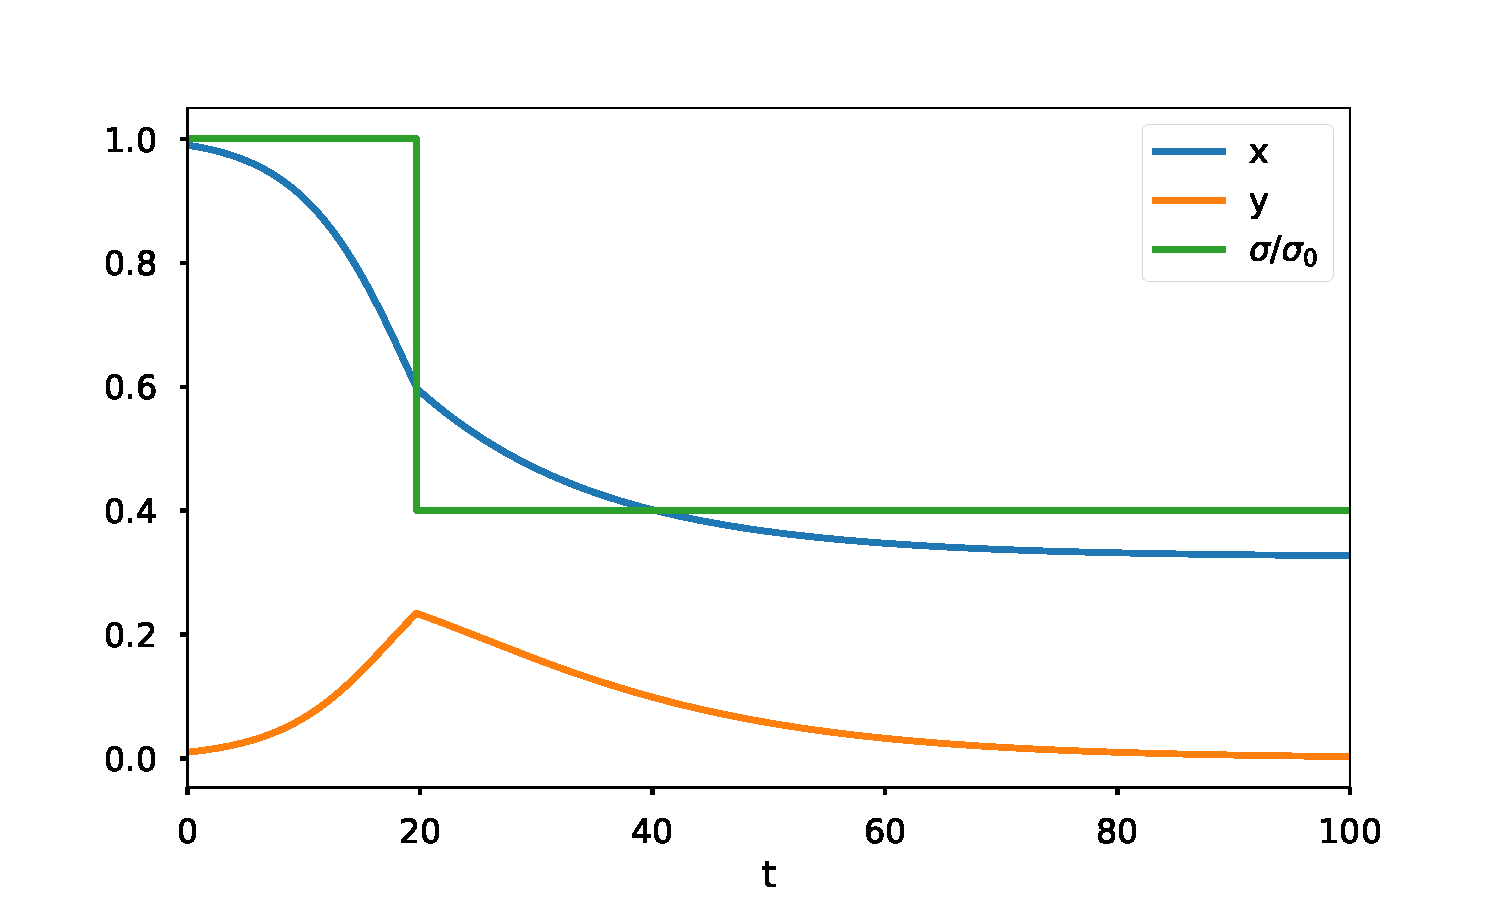
\includegraphics[width=0.65\textwidth]{figures/example2_time.pdf}}
    \subfigure[Trajectory in phase space]{\label{fig:example_2-xy}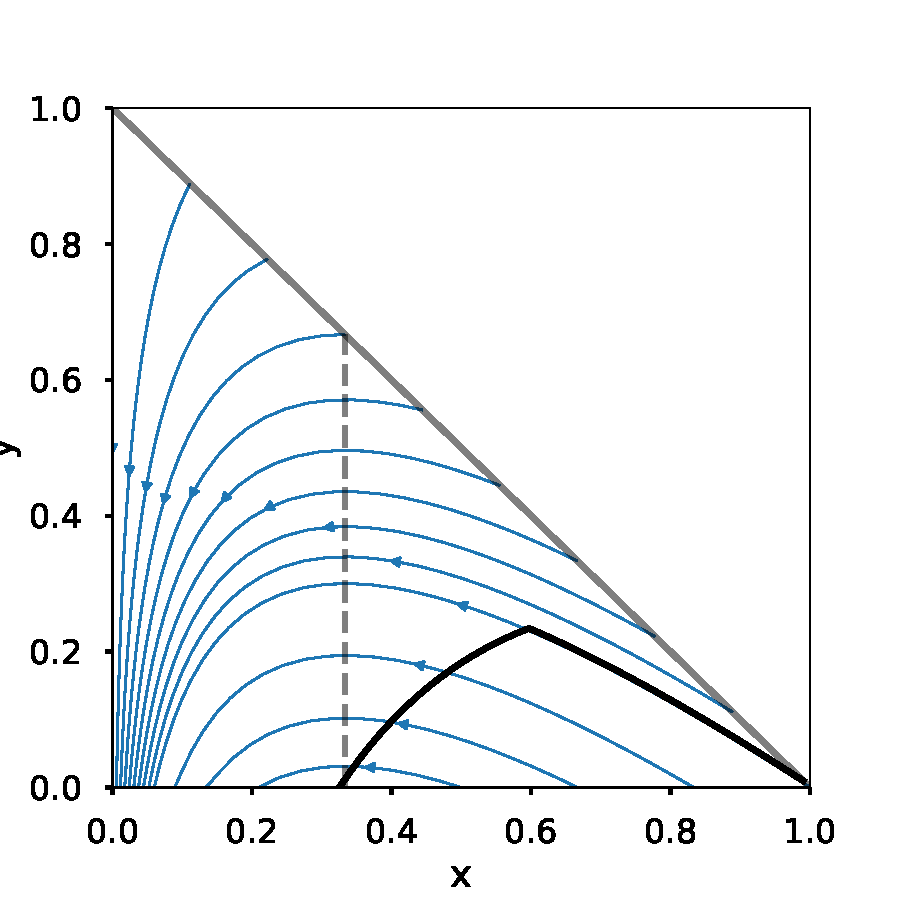
\includegraphics[width=0.34\textwidth]{figures/example2_xy.pdf}}
    \caption{Optimal solutions with $q(t)\le 0.6$.  Here $(x(0),y(0)) = (0.99,0.01)$, $\beta=0.3$, $\gamma=0.1$, and $T=100$.\label{fig:example_2}}
\end{figure}


\subsection{Minimizing hospital overflow}
The optimal solutions above may be unsatisfactory in practice for various reasons.
For instance, the number of people simultaneously infected just before the control
turns on may be too large to receive adequate medical care.  This is a major concern
with respect to the current COVID-19 crisis.  A natural objective is to keep
the number of infected below some threshold, corresponding for instance to the
number of hospital beds.  We thus consider the objective:
$$
    J = -\Sinf(x(T),y(T),\Rnot) + \int_0^T \left(c_2 (q(t))^2 + c_3 g(y-y_\text{max})\right) dt.
$$
Here $\ymax$ is the maximum number of hospital beds.
The function $g(v)$ should be nearly zero for $v<0$ and increase
in an approximately linear fashion for $v>0$.  For the purpose of having
a tractable control problem, it is also desirable that $g$ be differentiable.
We take
$$
g(v) = \frac{v}{1+e^{-10v}}.
$$

An example of an optimal solution is shown in Figure \ref{fig:min_hosp_1}, where
we consider the case of very low but non-zero cost of control ($c_2=2\times 10^{-5}$) and
high cost of hospital overflow ($c_3=200$).  As expected, $y(t)$ is generally
kept below $\ymax$, which is set to $0.1$ and
indicated with a horizontal dashed line.  The control is initially off, then turns on
to avoid hospital overflow, and then turns off again.  While the control is applied,
it is maintained at a level that keeps the value of $y(t)$ constant in time.

\begin{figure}
    \centering
    \subfigure[Solution and control vs. time]{\label{fig:minhosp1-time}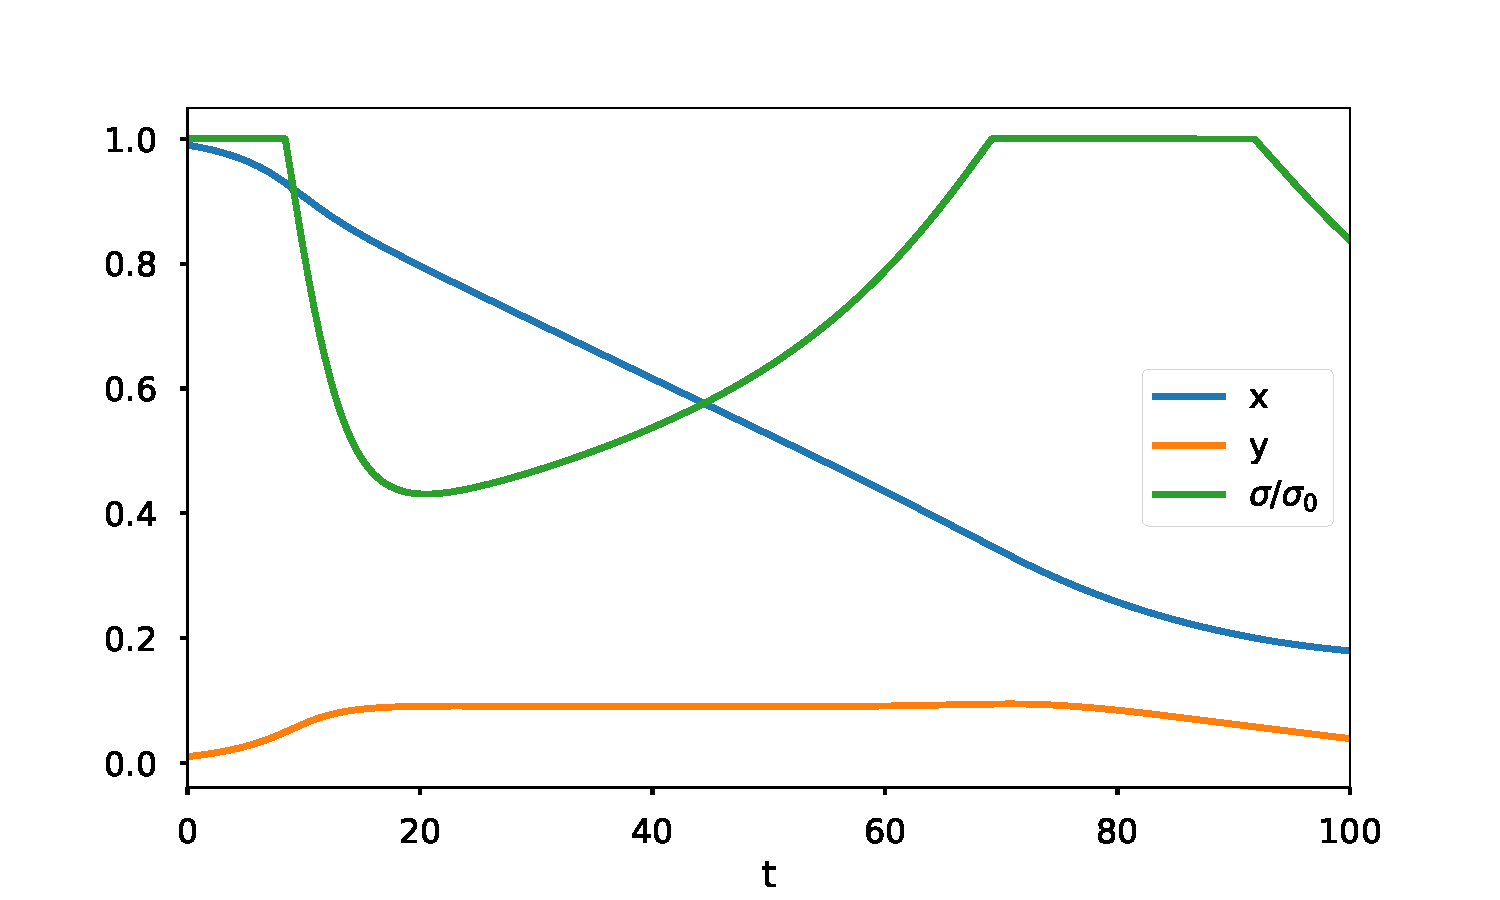
\includegraphics[width=0.65\textwidth]{figures/min_hosp_1_t.pdf}}
    \subfigure[Trajectory in phase space]{\label{fig:minhosp1-xy}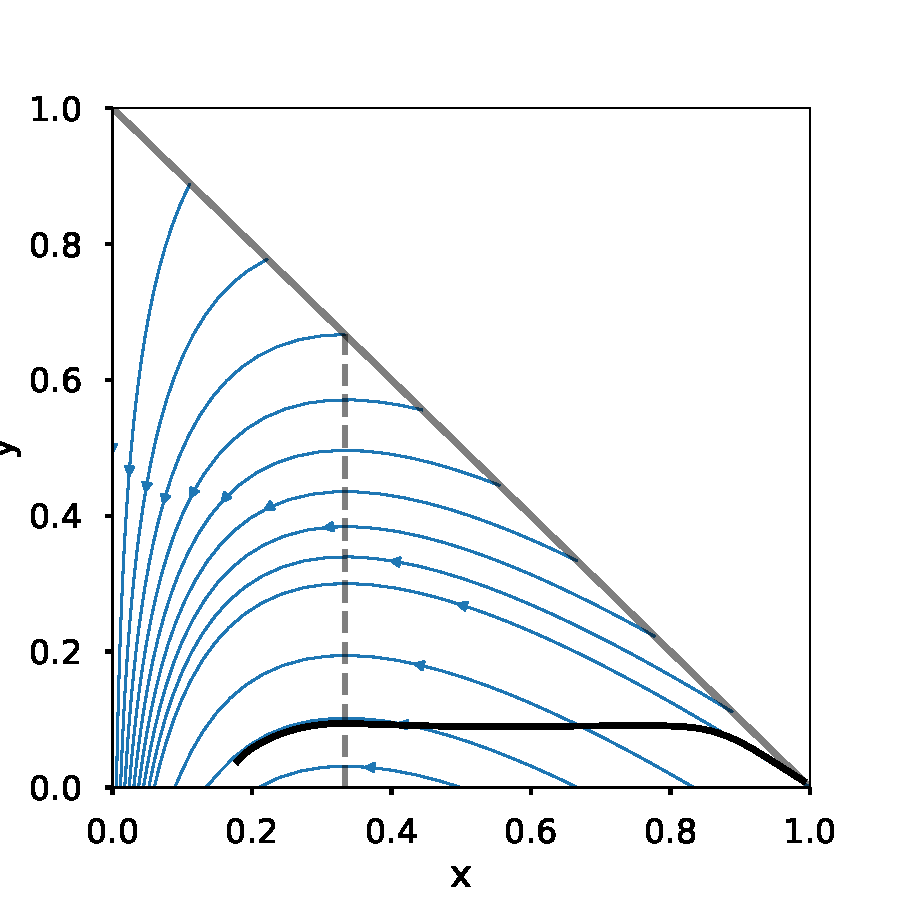
\includegraphics[width=0.34\textwidth]{figures/min_hosp_1_xy.pdf}}
    \caption{Optimal solutions with high cost for hospital overflow.  Here $(x(0),y(0)) = (0.99,0.01)$, $\beta=0.3$, $\gamma=0.1$, $T=100$,
        and $\ymax=0.1$.
        In the cost function, we take $c_2=2\times 10^{-5}$ (low cost of control) and $c_3=200$ (high cost of hospital overflow).\label{fig:min_hosp_1}}
\end{figure}

Figure \ref{fig:min_hosp_2} shows another example scenario in which the cost of hospital overflow ($c_3=10$)
and the cost of control ($c_2=10^{-3}$) are more comparable.  In this case the control is turned on and off gradually.

\begin{figure}
    \centering
    \subfigure[Solution and control vs. time]{\label{fig:minhosp2-time}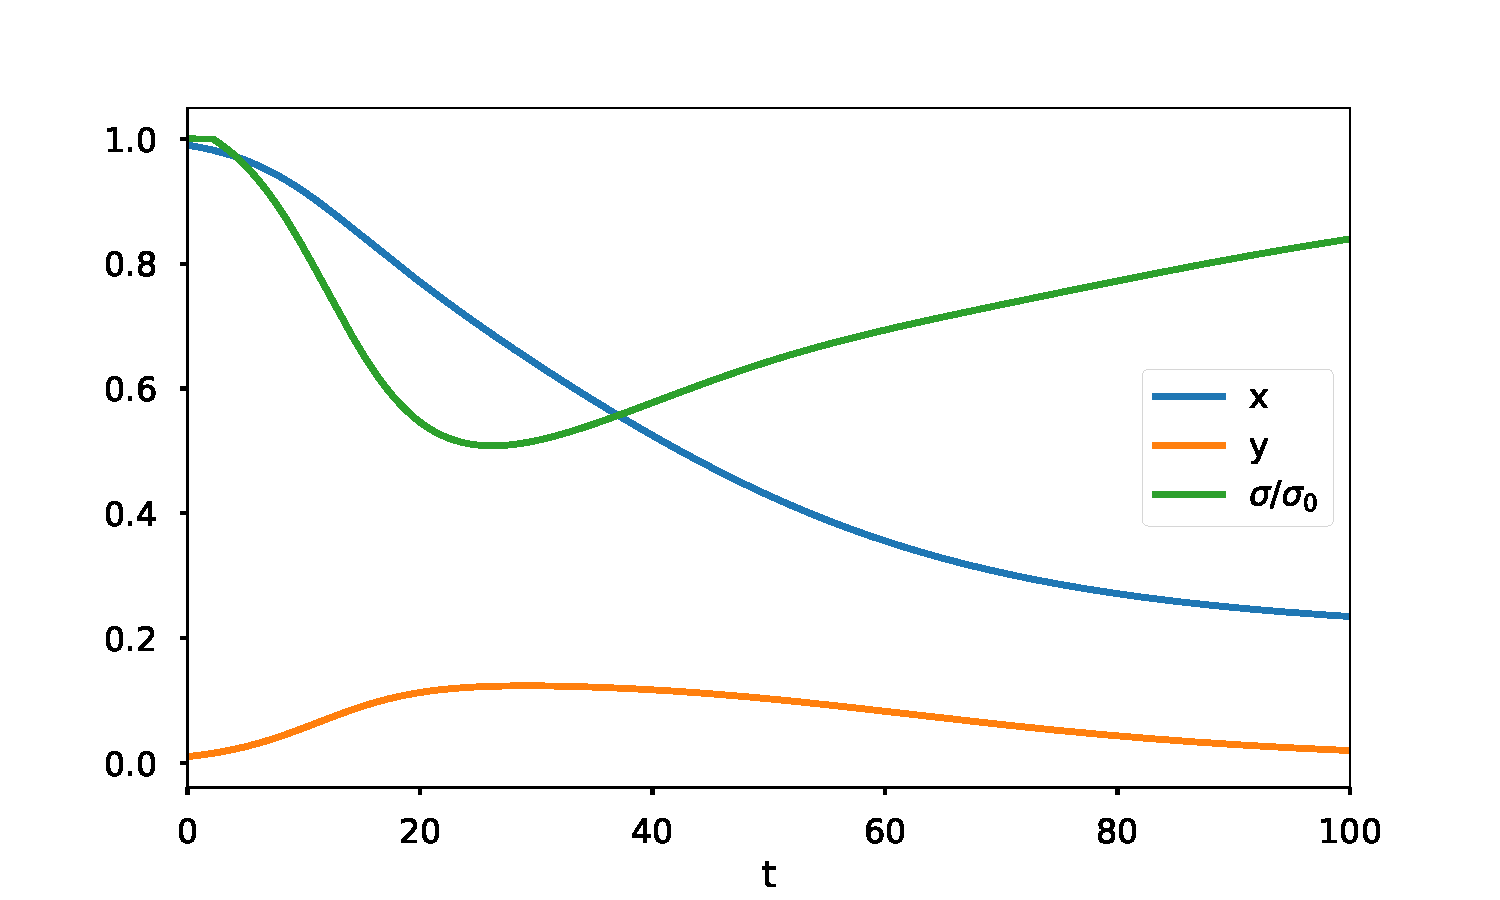
\includegraphics[width=0.65\textwidth]{figures/min_hosp_2_t.pdf}}
    \subfigure[Trajectory in phase space]{\label{fig:minhosp2-xy}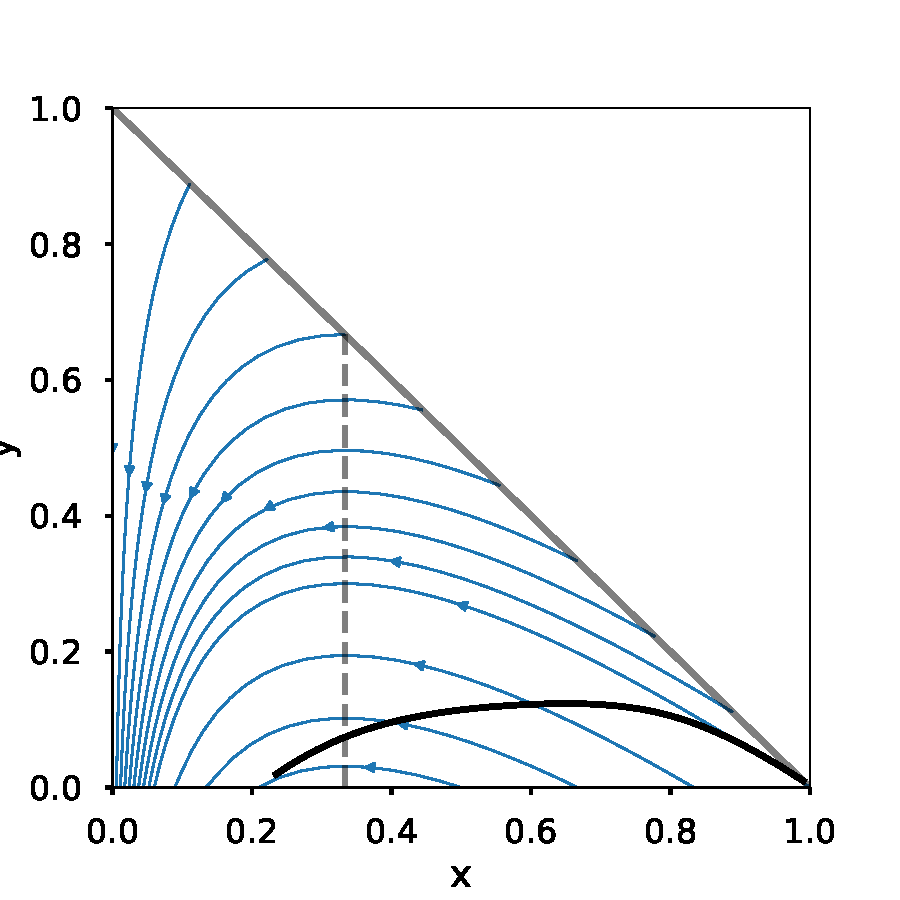
\includegraphics[width=0.34\textwidth]{figures/min_hosp_2_xy.pdf}}
    \caption{Optimal solutions with moderate cost for hospital overflow.  Here $(x(0),y(0)) = (0.99,0.01)$, $\beta=0.3$, $\gamma=0.1$, $T=100$,
        and $\ymax=0.1$.
        In the cost function, we take $c_2=10^{-3}$ and $c_3=10$.\label{fig:min_hosp_2}}
\end{figure}

\section{Conclusion}
We have studied, for an SIR model with a control on the rate of contact, the
problem of minimizing the eventually infected population in the long-time limit,
when the control can be apply only up to a finite time.  In the absence of any
cost of intervention, the optimal strategy is to apply no control until a
certain switching time, and then apply maximum control.  We have also considered
a range of other objective functions, including one in which a strong weight is
placed on avoiding large numbers of simultaneous infections.  In the latter case,
the control is turned on just before the threshold number of infections is reached,
and then maintained at a level just sufficient to avoid passing the threshold.

Although this work has focused on fundamental mathematical theory, there are
important implications that are relevant to real-world epidemics.  First,
observe that the optimal solutions obtained here, based on $\Sinf$, are
drastically different than those that would be obtained if the objective
were to maximize $x(T)$.  In the latter case, an optimal strategy over
short times is to apply very strong control from the outset.  But the long-term
outcome of such a strategy, if intervention cannot be maintained forever,
is simply to delay the epidemic.  This has been borne out in real epidemics.
A study of the 1918 influenza pandemic found no statistically significant
correlation between interventions and the eventual death toll in US cities
\cite{hatchett2007public}.  In simple terms, flattening the curve also
broadens the curve and may not have a substantial impact on the area under the
curve.

Real-world application of the strategies derived here would require
precise knowledge of the disease parameters, the current state of the
population, and the quantitative effect of specific NPIs, none of which
are readily available (or indeed capable of being characterized by a single
number).  Nevertheless, the general results obtained here provide insight
into what optimal intervention strategies and their consequences may look like.


\bibliographystyle{plain}
\bibliography{refs}

\end{document}
